%% LaTeX-Beamer template for KIT design
%% by Erik Burger, Christian Hammer
%% title picture by Klaus Krogmann
%%
%% version 2.1
%%
%% mostly compatible to KIT corporate design v2.0
%% http://intranet.kit.edu/gestaltungsrichtlinien.php
%%
%% Problems, bugs and comments to
%% burger@kit.edu

\documentclass[18pt]{beamer}

%% SLIDE FORMAT

% use 'beamerthemekit' for standard 4:3 ratio
% for widescreen slides (16:9), use 'beamerthemekitwide'

\usepackage{templates/beamerthemekit}
% \usepackage{templates/beamerthemekitwide}

%% TITLE PICTURE

% if a custom picture is to be used on the title page, copy it into the 'logos'
% directory, in the line below, replace 'mypicture' with the
% filename (without extension) and uncomment the following line
% (picture proportions: 63 : 20 for standard, 169 : 40 for wide
% *.eps format if you use latex+dvips+ps2pdf,
% *.jpg/*.png/*.pdf if you use pdflatex)

%\titleimage{mypicture}

%% TITLE LOGO

% for a custom logo on the front page, copy your file into the 'logos'
% directory, insert the filename in the line below and uncomment it

%\titlelogo{mylogo}
\titlelogo{empty_logo}

% (*.eps format if you use latex+dvips+ps2pdf,
% *.jpg/*.png/*.pdf if you use pdflatex)

%% TikZ INTEGRATION

% use these packages for PCM symbols and UML classes
% \usepackage{templates/tikzkit}
% \usepackage{templates/tikzuml}

% the presentation starts here

\title[Cosmic rays data center]{Current status of data center for cosmic rays \\based on KCDC}
\subtitle{GRID-2018, Dubna}
\author{Dmitriy Kostunin, Victoria Tokareva}

\institute{Institute for Nuclear Physics (IKP)}

\date{September 12, 2018}

% Bibliography

\usepackage[citestyle=authoryear,bibstyle=numeric,hyperref,backend=biber]{biblatex}
\addbibresource{templates/example.bib}
\bibhang1em

\begin{document}

% change the following line to "ngerman" for German style date and logos
\selectlanguage{english}

%title page
\begin{frame}
\titlepage
\end{frame}

%table of contents
\begin{frame}[allowframebreaks]{Outline}
Ориентировочный план действий:
\begin{itemize}
 \item Вводная:
 \begin{itemize}
 \item astroparticle phzsics и как это всё дофига важно
 \item тренды: больше станций или общие данные?
 \item итого: совместная российско-немецкая инцициатива
 \end{itemize}
 \item сравнение KASCADE и Tunka (почему должно быть интересно объединить данные, проблемы и решения):
 %обязательно сказать, что в астрофизике такое делается вперые (хотя в целом тема не нова), и мы работаем в столрону proof of work
 \begin{itemize}
    \item физика: в чем разница собираемых данных?
    \item разница по метаданным
    \item организация хранения: у KASCADE есть KCDC, и всё крайне аккурктно оргинизовано (рассказать, как),
    у Tunka все в процессе (оказывается, есть крутой слайд у Костюнина про это (5/13))
    \item обработка? общая она или раздельная? в чем разница? как мошла бы выглядеть общая схема обработки?
    \item как можно было бы организовать совместный быстрый доступ пользователей к данным/инструментам анализа?
    \item почему мы считаем, что эксперименты можно определить, и почему именно Tunka()?
 \end{itemize}
 \item Как мы думаем, это можно было бы сделать:
    \begin{itemize}
        \item MWS как идея
        %при объединении распрд. ресурсов возникает такое понятие, как интероперабельность системы. она может быть обеспечена на 3-х уровнях: организационном (т.е., руками), техническом (автоматизация процессов)  и семантическом
        \item какие-нибудь схематические догадки о том, как это все касается нас
        \item job workflow
        \item какую систему будем юзать?
\end{itemize}
\item А что уже сделанно к наст моменту?
    \begin{itemize}
     \item общая схема KCDC
     \item astroparticle.online
     \item описание метаданных
    \end{itemize}
\item Conclusion: мы собрались делать большое дело, у нас есть богатая история, много планов и даже чуть-чуть из них уже сделано. Следующим шагом проекта станет...
% \tableofcontents
\end{itemize}

\end{frame}

\begin{frame}{Introduction}
Вступление - такие вступление :)
Современная астрофизика представлена большим количеством экспериментов, которые изучают примерно одно и то же (а зачастую - и прям совсем одно и то же, в плане объекта), но по-разному - т.е., в разных природных условиях и с использованием разных типов детекторов.
Каждый год данных прибывает, и при этом общй дата пул ежегодно растет, как на дрожжах (см. картинку)

\begin{figure}[h]
\center{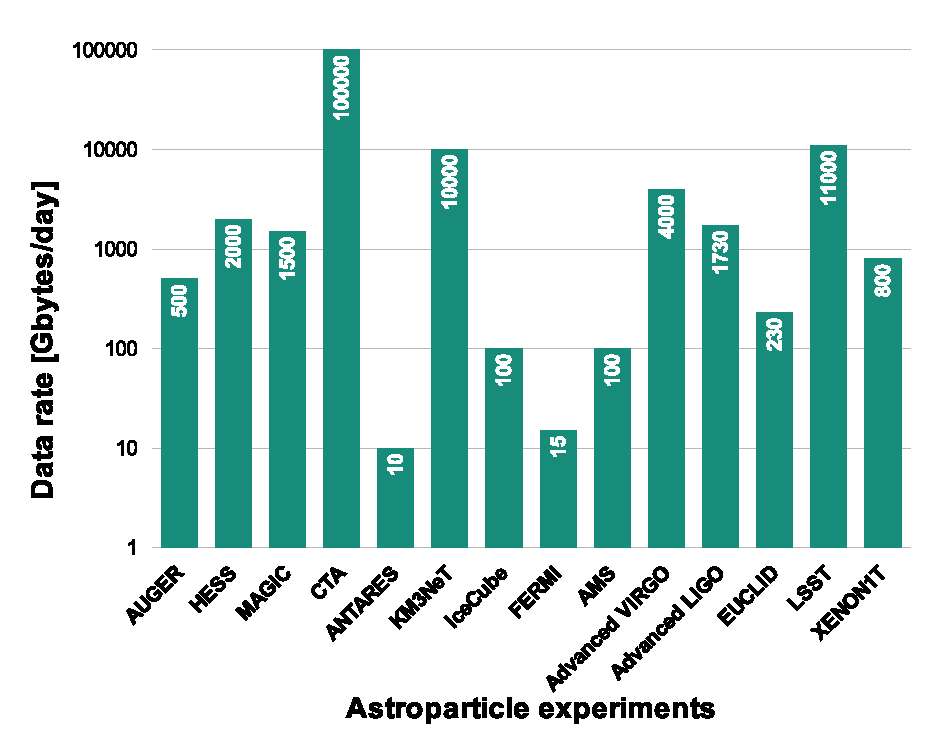
\includegraphics[width=1\linewidth]{"pics/appec_computing-diagram.jpg"}}
\caption{Данные от экспериментов в области астрофизики}
\label{ris:image}
\end{figure}

\end{frame}


\begin{frame}{\textcolor{kit-green100}{KRAD}: \textcolor{kit-green100}{K}arlsruhe-\textcolor{kit-green100}{R}ussian \textcolor{kit-green100}{A}stroparticle \textcolor{kit-green100}{D}ata Life Cycle}

Как можно догадаться по названию, являет совместным Российско-немецким проектом, включающим в себя с российской стороны такие инстиутты как ... (перечислить, какие)
Суть: создание единого центра обработки астрофизических данных.

\end{frame}


\section{Section 1}
\subsection{Subsection 1.1}
% \begin{frame}{Example slide A}
% \begin{itemize}
% \item PCM, Citation: \cite{becker2008a} %\language
% \pause
% \item Bullet point 2
% \item \dots
% \end{itemize}
% \end{frame}
%
% \subsection{Subsection 1.2}
% \begin{frame}{Example slide B}
% \begin{block}{Block 1}
% \begin{itemize}
% \item Bullet point 1
% \pause
% \item Bullet point 2
% \item \dots
% \end{itemize}
% \end{block}
% \end{frame}
%
% \section{Section 2}
% \begin{frame}{Example slide C}
% \begin{exampleblock}{Example 1}
% \begin{itemize}
% \item Bullet point 1
% \pause
% \item Bullet point 2
% \item \dots
% \end{itemize}
% \end{exampleblock}
% \end{frame}
%
% \begin{frame}{Example slide D}
% \begin{alertblock}{Alert 1}
% \begin{itemize}
% \item Bullet point 1
% \pause
% \item Bullet point 2
% \item \dots
% \end{itemize}
% \end{alertblock}
% \end{frame}
%
% \appendix
% \beginbackup
%
% \begin{frame}[allowframebreaks]{References}
% \printbibliography
% \end{frame}
%
% \backupend

\end{document}
